%approach etc aan de handvan de rq's?

%\item Which techniques are used by browsers to make concurrently visiting multiple URLs possible?
%\item Which APIs are used by web browsers to make HTTP requests and retrieve webpages?
%\item How can we link an HTTP request to its source URL without the modification of the used web browser?
%\item What extra information from the client's (running) machine can be used to augment the information gained from network traffic to make the tracking of malware to its source URL easier?

Now the outline of this project has been set, it has become time to look how the research questions can be answered. 

\subsection{API analysis}

\subsection{Algorithm}
\begin{figure}[h]
    \centering
    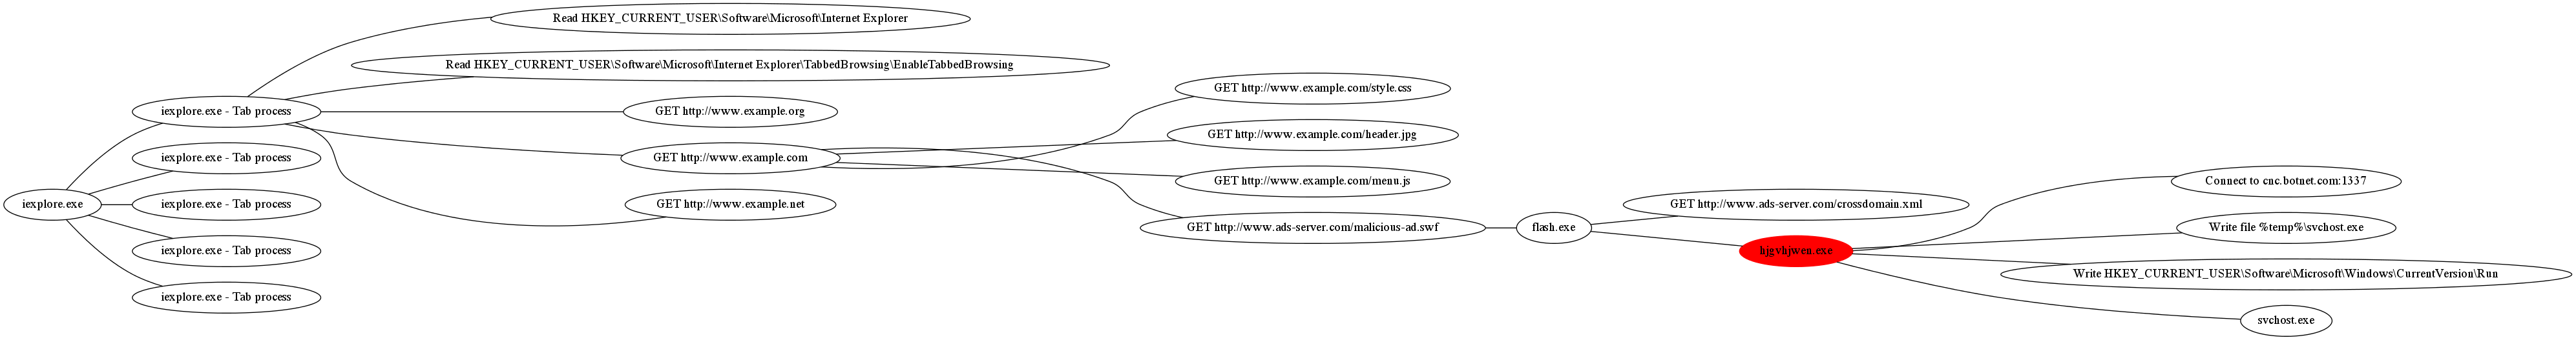
\includegraphics[width=17cm]{Images/alg_tree.png}
    \caption{An example of the graph}
    \label{fig:alg_tree}
\end{figure}

\subsubsection{Design considerations}

\subsubsection{Generic algorithm}

- Disconnected DAGs

1) Hooker schrijven voor elke browser die trafiek tussen Netwerk en Browser of in de browser zelf monitort en doorgeeft aan Cuckoo
2) DAG opstellen door de extra informatie te gebruiken in report.json
3) DAG interpreteren, nodes met enkel uitgaande edges zijn de beginnende URL
4) Kijken of er iets raar gebeurt in elk eiland
5) Reporting

\subsubsection{Platform-specific challenges}

Unix heeft geen handles zoals Windows maar meer files
	- FD's eigenlijk

\subsubsection{Alternative approaches}

- pcap / mitm
- tijd based
- aangepaste headers

\subsection{Proof of Concept}
	- Cuckoo aanpassen
		- Multiple URL support
		- Fixed Yara
	- Analyzer in Python
		- report.json parser
		- Commandline interface
			- Input: file, lijst op cli
			- Generic algorithm
			- Output: "No Malicious activity found", "URL xxxxx shows malicious activity: en dan wat korte informatie" 
		- 
